\chapter{Meiosis, Pencampuran Genetik, dan Pewarisan}\label{ch:b2:meiosis-heredity}

Dua orang tua bermata cokelat memperoleh seorang anak bermata biru, dan
tak seorang pun terkejut; dua anak dari orang tua yang sama tidak
pernah serupa, dan tak seorang pun terkejut pula. Kedua kenyataan itu
mengikuti satu proses yang sama. Pada pembuatan tiap sel telur dan tiap
sperma, sebuah sel yang memiliki dua salinan tiap kromosomnya
menyerahkan tepat satu salinan, yang dipilih secara acak, sesudah
membiarkan kedua salinannya bertukar ruas. Tiap pembuahan lalu
mempertemukan dua setengah perangkat yang belum pernah berjumpa. Bab
ini memerikan proses itu --- \omterm{def:b2:meiosis-heredity:meiosis}{meiosis} --- dan kaidah pewarisan yang
mengikutinya: nisbah Mendel, kekecualiannya, \omterm{def:b2:meiosis-heredity:linkage}{pautan} gen yang berbagi
satu kromosom dan peta yang digambar \omterm{def:b2:meiosis-heredity:linkage}{pautan} itu, serta pewarisan
istimewa \omterm{prop:b2:meiosis-heredity:sexlinked}{kromosom kelamin} dan organel.

\section{Meiosis}

\begin{definition}[Meiosis]\label{def:b2:meiosis-heredity:meiosis}
\index{meiosis}\index{haploid}\index{diploid}
Sebuah sel \emph{diploid} ($2n$) mengusung dua kromosom
\emph{homolog} tiap jenisnya, satu dari tiap tetuanya, serupa
kandungan gennya tetapi belum tentu serupa \omterm{def:b2:meiosis-heredity:vocabulary}{alelnya}. \emph{Meiosis}
adalah sepasang pembelahan yang mengubah satu sel diploid menjadi empat
sel \emph{haploid} ($n$), masing-masing dengan satu kromosom tiap
jenisnya. Ia didahului satu replikasi, sehingga tiap kromosomnya masuk
sebagai dua kromatid saudari; pembelahan pertamanya memisahkan
\emph{homolog} (reduksional), pembelahan keduanya memisahkan
\emph{kromatid saudari} (ekuasional), seperti yang dikerjakan mitosis.
Pada hewan meiosis membuat gamet; pada tumbuhan dan fungi ia membuat
spora (\cref{ch:b2:plant-life-cycles}); pada tiap organisme seksual ia
adalah langkah yang memerohkan cacah kromosomnya sehingga pembuahan
dapat melipatduakannya kembali.
\end{definition}

\begin{proposition}[Tahap-tahapnya]\label{prop:b2:meiosis-heredity:stages}
\index{profase I}\index{sinapsis kromosom}\index{kiasma}\index{pindah silang}
\emph{\omterm{prop:b2:meiosis-heredity:stages}{Profase I}} berlangsung lama dan di situlah pencampurannya
terjadi. Kromosom yang telah bereplikasi memadat; masing-masing
menemukan homolognya lalu berpasangan dengannya gen demi gen
(\emph{\omterm{prop:b2:meiosis-heredity:stages}{sinapsis kromosom}}), ditahan sebuah tangga protein, yaitu \emph{kompleks
sinaptonemal}, sehingga terbentuk sebuah \emph{bivalen} berisi empat
kromatid; kromatid bukan saudari putus lalu bersambung kembali pada
titik yang bersesuaian (\emph{\omterm{prop:b2:meiosis-heredity:stages}{pindah silang}}), satu sampai beberapa
kali tiap bivalennya; ketika kompleksnya melarut, homolognya tetap
melekat hanya pada titik pertukaran itu, yang terlihat sebagai
\emph{kiasma}. \emph{Metafase I}: bivalennya berbaris pada
gelendongnya, tiap pasangannya berarah acak --- homolog dari ibunya
menghadap satu kutub atau kutub yang lain secara bebas dari tiap
pasangan lainnya. \emph{Anafase I}: homolognya berpisah, sedangkan
kromatid saudarinya tetap bersama; tiap kutubnya menerima $n$ kromosom
yang masing-masing berkromatid dua. \emph{Telofase I} dan, biasanya
tanpa replikasi, \emph{\omterm{def:b2:meiosis-heredity:meiosis}{meiosis} II}: $n$ kromosomnya
berbaris satu-satu, kromatid saudarinya berpisah, dan terbentuklah
empat nukleus \omterm{def:b2:meiosis-heredity:meiosis}{haploid}. \omterm{def:b2:meiosis-heredity:meiosis}{Meiosis} I memakan waktu berjam-jam sampai
berpuluh tahun (oosit manusia berhenti pada \omterm{prop:b2:meiosis-heredity:stages}{profase I} sejak sebelum
lahir sampai ovulasi); \omterm{def:b2:meiosis-heredity:meiosis}{meiosis} II memakan satu jam.
\end{proposition}

\begin{omfigure}
\begin{tikzpicture}[every node/.style={font=\scriptsize}]
  % helper: cell outline at (x,y)
  \foreach \x/\lab in {0/{profase I: pemasangan, pindah silang}, 3.2/{metafase I: bivalen berjajar}, 6.4/{anafase I: homolog berpisah}, 9.6/{meiosis II: kromatid berpisah}}
    { \draw[thick] (\x+1.2,0) circle (1.15); \node[below, align=center, text width=2.8cm] at (\x+1.2,-1.2) {\lab}; }
  % prophase I: one bivalent with chiasma
  \draw[very thick, omDef] (0.8,-0.5) -- (0.8,0.5); \draw[very thick, omDef] (1.0,-0.5) -- (1.0,0.5);
  \draw[very thick, omThm] (1.4,-0.5) -- (1.4,0.5); \draw[very thick, omThm] (1.6,-0.5) -- (1.6,0.5);
  \draw[very thick, omDef] (1.0,0.1) -- (1.4,-0.1); \draw[very thick, omThm] (1.4,0.1) -- (1.0,-0.1);
  \fill[white] (0.9,-0.03) rectangle (1.5,0.03);
  \draw[very thick, omDef] (1.0,0.1) -- (1.4,-0.1); \draw[very thick, omThm] (1.4,0.1) -- (1.0,-0.1);
  \node[omExo!60!black] at (1.2,-0.85) {kiasma};
  % metaphase I: two bivalents on the plate, spindle
  \begin{scope}[xshift=3.2cm]
    \draw[gray, dashed] (1.2,-1.0) -- (1.2,1.0);
    \foreach \y in {0.45,-0.45} {
      \draw[very thick, omDef] (0.95,\y-0.25) -- (0.95,\y+0.25); \draw[very thick, omDef] (1.08,\y-0.25) -- (1.08,\y+0.25);
      \draw[very thick, omThm] (1.32,\y-0.25) -- (1.32,\y+0.25); \draw[very thick, omThm] (1.45,\y-0.25) -- (1.45,\y+0.25);
    }
    \draw[gray] (0.15,0) -- (0.95,0.45); \draw[gray] (0.15,0) -- (0.95,-0.45);
    \draw[gray] (2.25,0) -- (1.45,0.45); \draw[gray] (2.25,0) -- (1.45,-0.45);
  \end{scope}
  % anaphase I
  \begin{scope}[xshift=6.4cm]
    \foreach \y in {0.45,-0.45} {
      \draw[very thick, omDef] (0.45,\y-0.25) -- (0.45,\y+0.25); \draw[very thick, omDef] (0.58,\y-0.25) -- (0.58,\y+0.25);
      \draw[very thick, omThm] (1.82,\y-0.25) -- (1.82,\y+0.25); \draw[very thick, omThm] (1.95,\y-0.25) -- (1.95,\y+0.25);
    }
    \draw[->, gray] (1.2,0) -- (0.75,0); \draw[->, gray] (1.2,0) -- (1.65,0);
  \end{scope}
  % meiosis II: four cells
  \begin{scope}[xshift=9.6cm]
    \foreach \p/\c in {(0.75,0.5)/omDef,(1.65,0.5)/omDef,(0.75,-0.5)/omThm,(1.65,-0.5)/omThm} {
      \draw[thick, gray!60] \p circle (0.38);
      \draw[very thick, \c] \p ++(-0.12,-0.2) -- ++(0,0.4);
      \draw[very thick, \c] \p ++(0.12,-0.2) -- ++(0,0.4);
    }
  \end{scope}
\end{tikzpicture}

{\small \omterm{def:b2:meiosis-heredity:meiosis}{Meiosis} bagi dua pasang homolog (biru dari ibu, merah dari
ayah, masing-masing berkromatid dua). Homolognya berpasangan dan
bertukar ruas pada \omterm{prop:b2:meiosis-heredity:stages}{profase I}, berjajar sebagai bivalen pada metafase I,
lalu berpisah pada anafase I; \omterm{def:b2:meiosis-heredity:meiosis}{meiosis} II memisahkan kromatidnya menjadi
empat sel \omterm{def:b2:meiosis-heredity:meiosis}{haploid}.}
\end{omfigure}

\begin{omfigure}
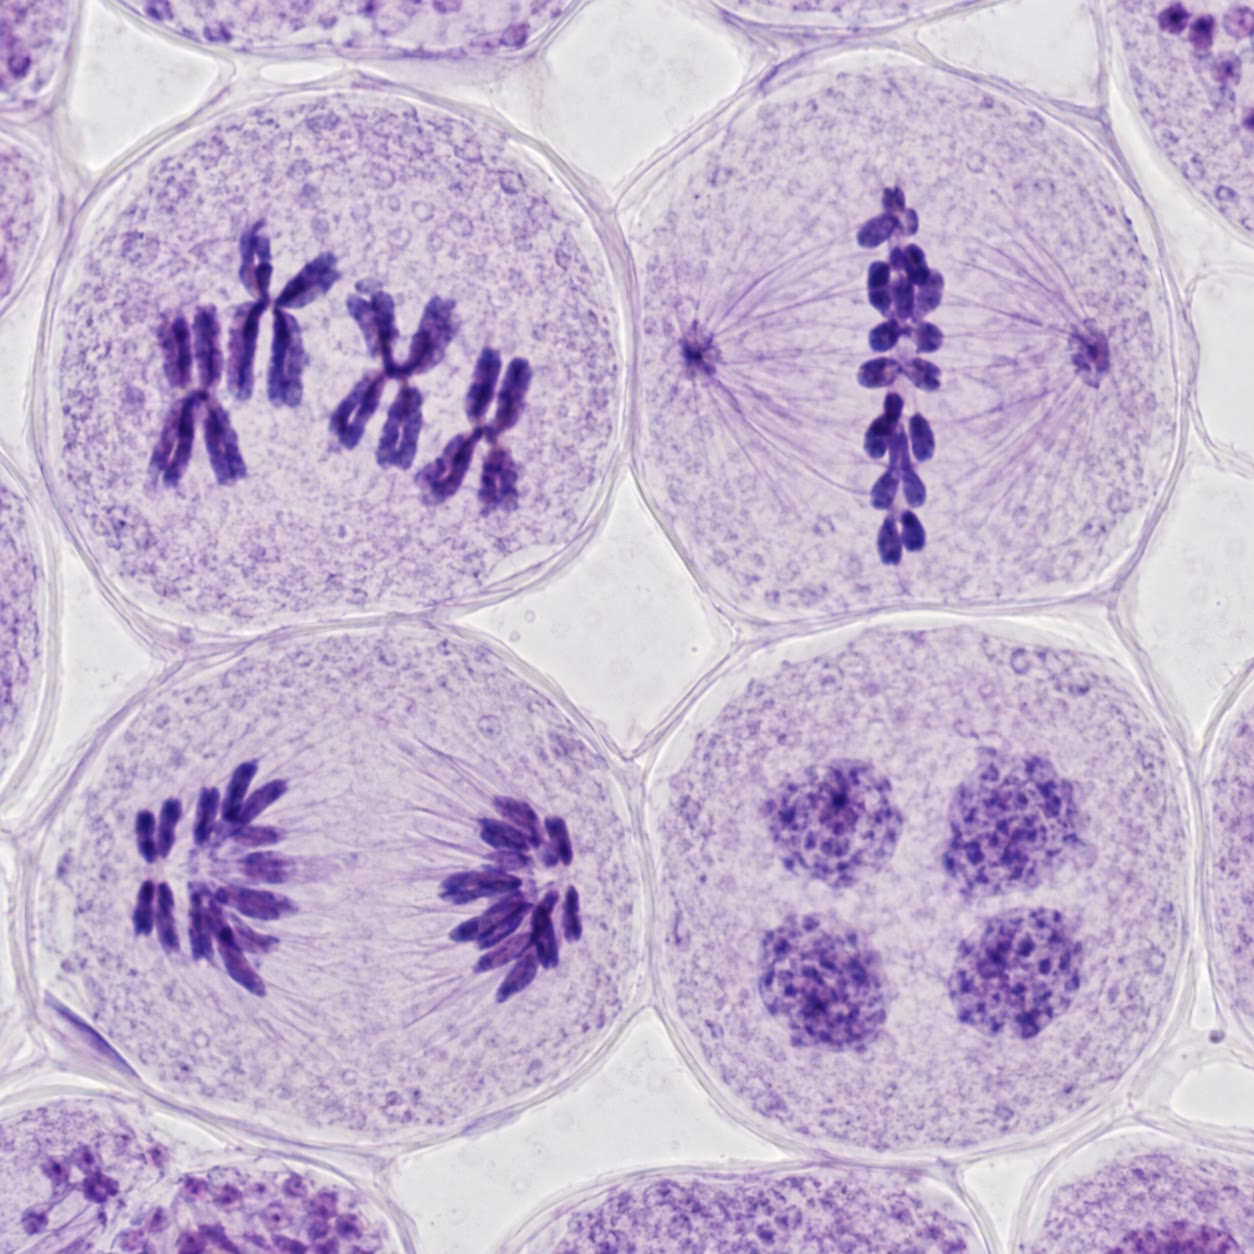
\includegraphics[width=0.5\linewidth]{images/book4/ai/b4-04-lily-meiosis.jpg}

{\small \omterm{def:b2:meiosis-heredity:meiosis}{Meiosis} di dalam kepala sari bunga bakung: bivalen pada akhir
\omterm{prop:b2:meiosis-heredity:stages}{profase I}, sebuah lempeng metafase I, anafase I, dan keempat nukleus
sebuah tetrad.}
\end{omfigure}

\begin{theorem}[Seberapa banyak pencampuran yang dibuat meiosis]\label{thm:b2:meiosis-heredity:mixing}
\index{pemilahan bebas}\index{rekombinasi genetik}
Bagi organisme dengan $n$ pasang kromosom, arah acak bivalennya pada
metafase I menghasilkan $2^n$ gabungan kromosom ibu dan ayah yang
mungkin di dalam sebuah gamet --- $2^{23} \approx 8.4$ juta pada
manusia --- dan $2^{2n}$ di dalam sebuah zigot. \omterm{prop:b2:meiosis-heredity:stages}{Pindah silang}
melipatgandakan angka ini: dengan kira-kira $k$ kiasma tiap bivalennya,
masing-masing pada kedudukan yang berubah-ubah, cacah gamet yang
berbeda menjadi tak terbatas secara efektif, dan tidak ada dua gamet
seseorang yang pernah sama. \emph{Rekombinasi} --- gabungan \omterm{def:b2:meiosis-heredity:vocabulary}{alel} yang
baru --- muncul dari keduanya: \omterm{thm:b2:meiosis-heredity:mixing}{pemilahan bebas} mengocok ulang
kromosom utuh, \omterm{prop:b2:meiosis-heredity:stages}{pindah silang} mengocok ulang gen di dalam satu
kromosom.
\end{theorem}
\begin{proof}
Tiap bivalennya berarah secara bebas dengan dua hasil, sehingga $n$
bivalen memberi $2^n$ gabungan yang semuanya sama mungkin. Masing-masing
dari kedua tetuanya menyumbang satu gamet semacam itu, sehingga zigotnya
memiliki $2^n\times
2^n$ gabungan. Sebuah \omterm{prop:b2:meiosis-heredity:stages}{pindah silang} pada kedudukan yang berbeda di
dalam kromosom berisi $L$ pasangan basa dapat menghasilkan kromatid
rekombinan yang berbeda seorde $L$ tiap bivalennya, sehingga cacah
hasil yang berbeda tumbuh seperti $L^k$ tiap kromosomnya, yang sangat
besar bagi $L \sim 10^8$.
\end{proof}
\begin{proof}[Bukti eksperimental]
Creighton dan McClintock (1931) memakai kromosom 9 jagung yang
mengusung dua tanda sitologi yang terlihat (sebuah bonggol pada satu
ujungnya, sebuah ruas tertranslokasi pada ujung yang lain) dan dua gen
di antaranya (biji berwarna/tak berwarna, endosperma pulut/bertepung).
Di antara keturunannya, tiap tumbuhan dengan sepasang \omterm{def:b2:meiosis-heredity:vocabulary}{alel} hasil
rekombinasi juga memiliki sepasang tanda sitologi hasil rekombinasi ---
bonggol tanpa translokasi atau sebaliknya --- yang membuktikan bahwa
\omterm{thm:b2:meiosis-heredity:mixing}{rekombinasi genetik} adalah pertukaran ruas kromosom secara fisik.
\end{proof}

\begin{omfigure}
\begin{tikzpicture}[every node/.style={font=\scriptsize}]
  \foreach \dx/\lab/\ca/\cb/\gam in {0/{arah 1}/omDef/omThm/{gamet AB dan ab}, 6.2/{arah 2}/omThm/omDef/{gamet Ab dan aB}} {
    \begin{scope}[xshift=\dx cm]
      \draw[gray, dashed] (0,-1.1) -- (3.2,-1.1);
      \node[anchor=south] at (1.6,0.6) {\lab};
      % pair 1 (long): A above the plate, a below
      \draw[very thick, omDef] (0.7,-0.95) -- (0.7,-0.25); \node[omDef, anchor=south] at (0.7,-0.2) {A};
      \draw[very thick, omThm] (0.7,-1.25) -- (0.7,-1.95); \node[omThm, anchor=north] at (0.7,-2.0) {a};
      % pair 2 (short): B or b above depending on orientation
      \draw[very thick, \ca] (2.3,-0.85) -- (2.3,-0.35);
      \draw[very thick, \cb] (2.3,-1.35) -- (2.3,-1.85);
      \node[anchor=north] at (1.6,-2.4) {\gam};
    \end{scope}
  }
  \node[omDef, anchor=south] at (2.3,-0.3) {B}; \node[omThm, anchor=north] at (2.3,-1.9) {b};
  \node[omThm, anchor=south] at (8.5,-0.3) {b}; \node[omDef, anchor=north] at (8.5,-1.9) {B};
  \node[anchor=north, align=center] at (4.7,-3.0) {tiap arahnya sama mungkin:\\gamet AB, ab, Ab, aB sama banyak --- pemilahan bebas};
\end{tikzpicture}

{\small \omterm{thm:b2:meiosis-heredity:mixing}{Pemilahan bebas}. Bagi dua pasang kromosom (A/a pada satu
pasang, B/b pada pasang yang lain), kedua arah bivalennya yang mungkin
pada metafase I sama-sama mungkin, sehingga keempat gabungan \omterm{def:b2:meiosis-heredity:vocabulary}{alelnya}
muncul sama banyak di antara gametnya.}
\end{omfigure}

\section{Analisis Mendel}

\begin{definition}[Kosakata persilangan]\label{def:b2:meiosis-heredity:vocabulary}
\index{alel}\index{genotipe}\index{fenotipe}\index{dominan}%
\index{resesif}\index{homozigot}\index{heterozigot}
Sebuah \emph{gen} adalah seruas kromosom; \emph{alel}nya adalah varian
urutannya; \emph{lokus}nya adalah kedudukannya. Seorang individu
\omterm{def:b2:meiosis-heredity:meiosis}{diploid} mengusung dua alel pada tiap lokusnya: \emph{genotipe}nya
bersifat \emph{homozigot} ($AA$, $aa$) atau \emph{heterozigot} ($Aa$).
\emph{Fenotipe}nya adalah ciri yang teramati. Sebuah alel disebut
\emph{dominan} kalau heterozigotnya menampakkan fenotipenya, dan
\emph{resesif} kalau ia hanya tampak pada homozigotnya; pembedaan itu
adalah sifat sepasang alel dan sifat ciri yang diamati, bukan sifat
alelnya sendiri --- sebagian besar alel resesif adalah alel yang
kehilangan fungsi, tersembunyi karena satu salinan yang bekerja sudah
cukup. Sebuah \emph{galur murni} berbiak sejati (homozigot); sebuah
\emph{persilangan uji} mengawinkan individu berfenotipe dominan dengan
sebuah homozigot resesif, sehingga keturunannya menyingkapkan alel
gametnya secara langsung.
\end{definition}

\begin{theorem}[Nisbah Mendel]\label{thm:b2:meiosis-heredity:mendel}
\index{hukum Mendel}\index{persilangan monohibrid}\index{persilangan dihibrid}
Karena kedua \omterm{def:b2:meiosis-heredity:vocabulary}{alel} sebuah \omterm{def:b2:meiosis-heredity:vocabulary}{heterozigot} $Aa$ memilah ke dalam gamet yang
berbeda dalam jumlah yang sama (anafase I), sebuah persilangan
\emph{monohibrid} $Aa \times Aa$ memberi
\omterm{def:b2:meiosis-heredity:vocabulary}{genotipe} $\tfrac14 AA : \tfrac12 Aa :
\tfrac14 aa$, dan \omterm{def:b2:meiosis-heredity:vocabulary}{fenotipe} $3 : 1$ kalau $A$ \omterm{def:b2:meiosis-heredity:vocabulary}{dominan}; persilangan uji
$Aa \times aa$ memberi $1 : 1$. Karena \omterm{def:b2:meiosis-heredity:vocabulary}{alel} gen pada kromosom yang
berbeda memilah secara bebas (metafase I), sebuah \emph{dihibrid}
$AaBb$ membuat empat macam gamet dalam jumlah yang sama dan
persilangan $AaBb \times AaBb$ memberi \omterm{def:b2:meiosis-heredity:vocabulary}{fenotipe} $9 : 3 : 3 : 1$,
sedangkan persilangan uji $AaBb \times aabb$ memberi $1 : 1 : 1 : 1$.
Bagi $k$ lokus \omterm{def:b2:meiosis-heredity:vocabulary}{heterozigot} yang saling bebas, cacah macam gametnya
adalah $2^k$ dan nisbah \omterm{def:b2:meiosis-heredity:vocabulary}{fenotipenya} adalah hasil kali $k$ nisbah
$3 : 1$.
\end{theorem}
\begin{proof}
Pemilahan: gamet \omterm{def:b2:meiosis-heredity:vocabulary}{heterozigotnya} adalah $\tfrac12 A$,
$\tfrac12 a$; dengan pembuahan acak, \omterm{def:b2:meiosis-heredity:vocabulary}{genotipe} zigotnya adalah hasil
kali $(\tfrac12 A + \tfrac12 a)^2 = \tfrac14 AA + \tfrac12 Aa +
\tfrac14 aa$. Kebebasan: gamet $AaBb$ adalah $(\tfrac12 A
+ \tfrac12 a)(\tfrac12 B + \tfrac12 b)$, empat macam pada $\tfrac14$;
\omterm{def:b2:meiosis-heredity:vocabulary}{fenotipe} dihibridnya mengalikan $(\tfrac34 A\_ + \tfrac14 aa)
(\tfrac34 B\_ + \tfrac14 bb)$, sehingga memberi
$\tfrac{9}{16}, \tfrac{3}{16},
\tfrac{3}{16}, \tfrac{1}{16}$. Tiap faktornya adalah
satu \omterm{thm:b2:meiosis-heredity:mixing}{pemilahan bebas}, sehingga $k$ lokus memberi hasil kali $k$ faktor.
\end{proof}
\begin{proof}[Bukti eksperimental]
Mendel (1866) menyilangkan galur murni kacang ercis yang berbeda dalam
satu ciri --- biji bulat atau berkerut, kotiledon kuning atau hijau,
bunga ungu atau putih, batang tinggi atau kerdil, dan tiga ciri lain
--- lalu mendapati pada tiap kasusnya generasi pertama yang seragam dan
generasi kedua yang memilah mendekati $3 : 1$: 5474 bulat berbanding
1850 berkerut ($2.96 :
1$), 6022 kuning berbanding 2001 hijau ($3.01 : 1$), 705 ungu
berbanding 224 putih ($3.15 : 1$). Pada persilangan dua ciri ia
mendapati $315 : 108 : 101 :
32$ ($9 : 3 : 3 : 1$), dan dengan menumbuhkan generasi keduanya ia
menunjukkan bahwa golongan \omterm{def:b2:meiosis-heredity:vocabulary}{dominannya} terdiri atas dua macam,
sepertiganya murni dan dua pertiganya memilah. Kromosom yang
menjelaskan nisbahnya baru ditemukan empat puluh tahun kemudian.
\end{proof}

\begin{omfigure}
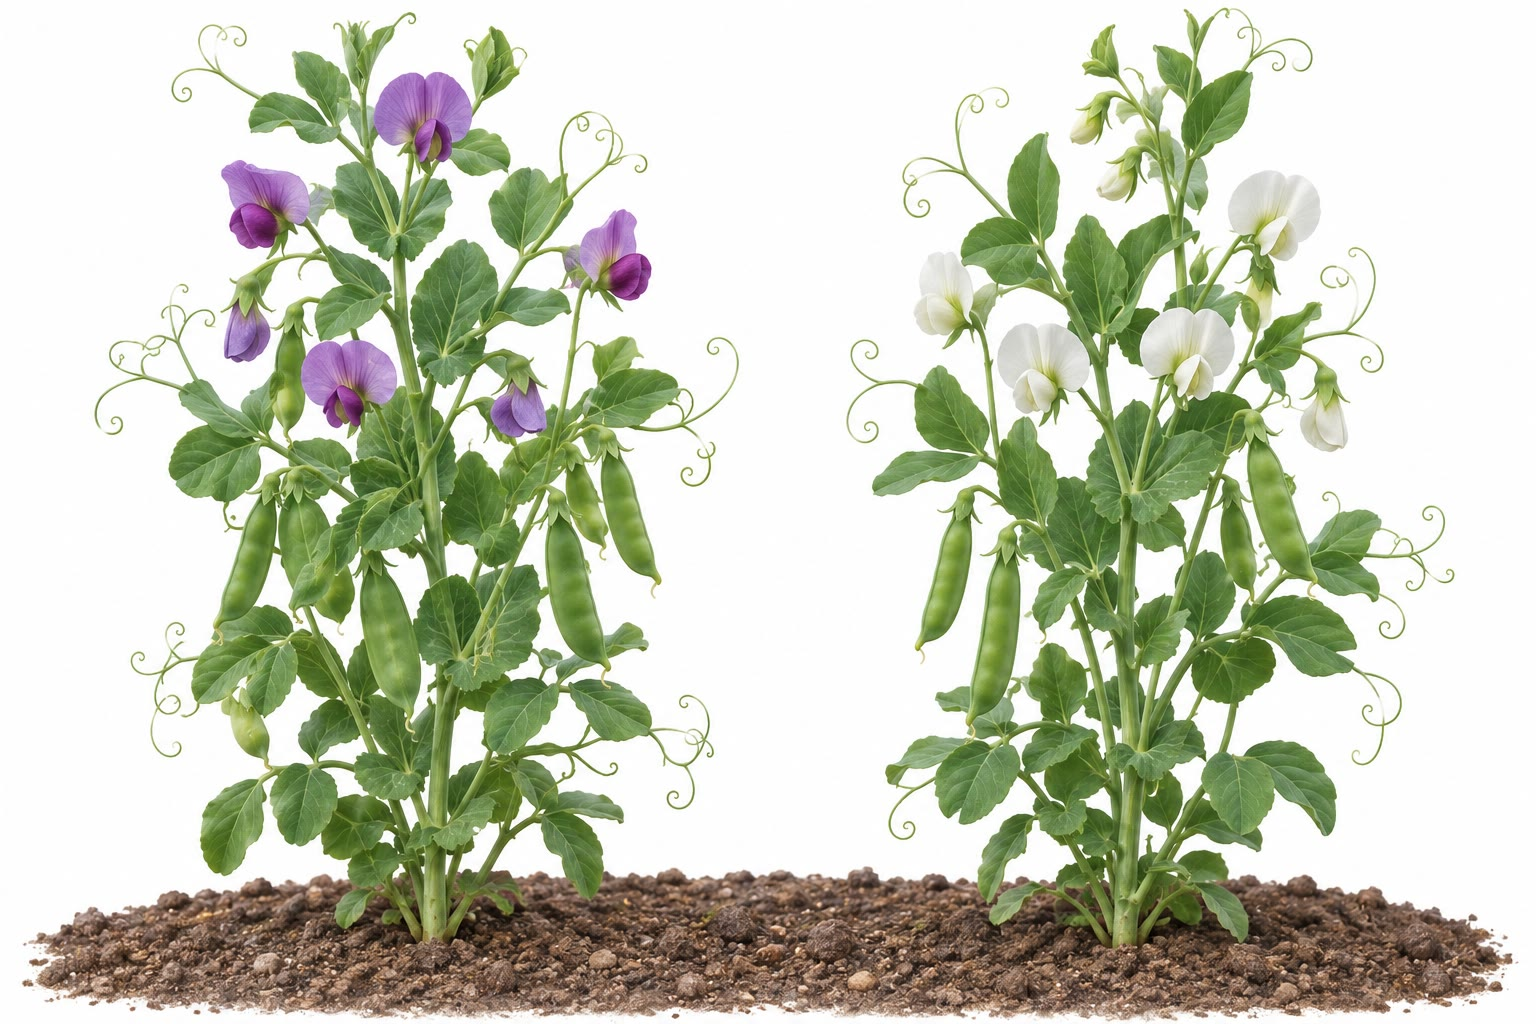
\includegraphics[width=0.58\linewidth]{images/book4/ai/b4-04-pea-flowers.jpg}

{\small Tumbuhan kacang ercis berbunga ungu dan berbunga putih: salah
satu dari tujuh pasang ciri yang di atasnya Mendel mendirikan genetika.
Hibrid berbunga ungu, kalau diserbuki sendiri, memberi kira-kira tiga
ungu berbanding satu putih.}
\end{omfigure}

\begin{method}[Menguji sebuah nisbah dengan $\chi^2$]\label{met:b2:meiosis-heredity:chisquare}
\index{uji khi-kuadrat}
Untuk memutuskan apakah cacah amatan $O_i$ cocok dengan nisbah yang
dihipotesiskan:
\begin{enumerate}
  \item Hitunglah cacah harapan $E_i$ dari nisbahnya dan dari
        jumlahnya.
  \item Hitunglah $\chi^2 = \sum_i (O_i - E_i)^2/E_i$.
  \item Cacahlah derajat kebebasannya: cacah golongannya dikurangi
        satu.
  \item Bandingkan dengan nilai kritisnya pada taraf \qty{5}{\%}:
        $3.84$ bagi 1 derajat kebebasan, $5.99$ bagi 2, $7.81$ bagi 3,
        $9.49$ bagi 4. Kalau $\chi^2$ berada di bawahnya, datanya
        sepadan dengan nisbahnya; kalau di atasnya, nisbahnya ditolak
        --- simpangan sebesar itu akan muncul secara kebetulan pada
        kurang dari satu percobaan dari dua puluh.
\end{enumerate}
Bagi bunga Mendel, $705 : 224$ terhadap $3 : 1$: $E = 696.75,
232.25$; $\chi^2 = 0.098 + 0.293 = 0.39 < 3.84$. (Sebaran di balik
nilai kritisnya diturunkan dalam statistika seri matematika; di sini
tabelnya sekadar sebuah alat.)
\end{method}

\begin{proposition}[Di luar nisbah yang sederhana]\label{prop:b2:meiosis-heredity:extensions}
\index{dominansi tak penuh}\index{kodominansi}\index{epistasis}\index{alel letal}
Nisbahnya berubah, tetapi mekanismenya tidak, ketika: \omterm{def:b2:meiosis-heredity:vocabulary}{alelnya}
memperlihatkan \emph{\omterm{prop:b2:meiosis-heredity:extensions}{dominansi tak penuh}} (snapdragon merah $\times$
putih memberi merah jambu, dan generasi keduanya $1 : 2 : 1$); \omterm{def:b2:meiosis-heredity:vocabulary}{alelnya}
bersifat \emph{kodominan}, keduanya terungkap (golongan darah $AB$:
\omterm{def:b2:meiosis-heredity:vocabulary}{heterozigot} $I^AI^B$ membuat kedua antigennya; sebuah lokus dapat
memiliki \emph{\omterm{def:b2:meiosis-heredity:vocabulary}{alel} ganda}, $I^A$, $I^B$, $i$); sebuah \omterm{def:b2:meiosis-heredity:vocabulary}{alel} bersifat
\emph{letal} ketika \omterm{def:b2:meiosis-heredity:vocabulary}{homozigot} (mencit kuning: kuning $\times$ kuning
memberi $2$ kuning berbanding $1$ agouti, karena $\tfrac14 YY$ mati
sebagai embrio); dua gen bekerja dalam satu lintasan
(\emph{epistasis}: dalam persilangan $9 : 3 : 3 : 1$, \omterm{def:b2:meiosis-heredity:vocabulary}{resesif} ganda
dan salah satu \omterm{def:b2:meiosis-heredity:vocabulary}{resesif} tunggal dapat tak terbedakan, sehingga memberi
$9 : 3 : 4$, seperti pada mencit albino, atau kedua \omterm{def:b2:meiosis-heredity:vocabulary}{dominannya} dapat
sama-sama dibutuhkan bagi \omterm{def:b2:meiosis-heredity:vocabulary}{fenotipenya}, sehingga memberi $9 : 7$,
seperti pada kacang manis ungu yang membutuhkan dua enzim untuk membuat
pigmennya); banyak gen yang masing-masing menambahkan sedikit pada ciri
yang sinambung (tinggi, hasil panen), yang menjadi genetika kuantitatif
\cref{ch:b2:population-genetics}. Membaca sebuah nisbah kembali menuju
mekanismenya adalah keterampilan sehari-hari genetika.
\end{proposition}

\section{Pautan dan peta genetik}

\begin{definition}[Pautan dan frekuensi rekombinasi]\label{def:b2:meiosis-heredity:linkage}
\index{pautan}\index{frekuensi rekombinasi}\index{sentimorgan}
Dua gen pada kromosom yang sama disebut \emph{terpaut}: \omterm{def:b2:meiosis-heredity:vocabulary}{alelnya}
cenderung mengembara bersama ke dalam gametnya, dan sebuah dihibrid
$AB/ab$ membuat gamet \emph{tetua} ($AB$, $ab$) lebih banyak daripada
gamet \emph{rekombinan} ($Ab$, $aB$). Rekombinan muncul hanya kalau
sebuah \omterm{prop:b2:meiosis-heredity:stages}{pindah silang} jatuh di antara kedua lokusnya, sehingga
frekuensinya $r$ --- yang dicacah langsung dalam sebuah persilangan uji
--- mengukur jaraknya: $r$ terentang dari 0 (pautan sempurna) sampai
$\tfrac12$ (gen yang begitu berjauhan, atau berada pada kromosom yang
berbeda, sehingga memilah secara bebas). Satuan \emph{jarak peta}nya
adalah \emph{sentimorgan} (cM): \qty{1}{cM} adalah rekombinasi
\qty{1}{\%} bagi gen yang terpaut rapat; pada manusia \qty{1}{cM}
kira-kira sejuta pasangan basa. Pautan adalah bukti pertama bahwa gen
terletak dalam sebuah garis pada kromosomnya.
\end{definition}
\begin{proof}[Bukti eksperimental]
Morgan (1911) mendapati bahwa gen mata putih dan sayap mungil pada
lalat, keduanya pada kromosom X, tidak memilah secara bebas: sebuah
persilangan uji memberi \qty{37}{\%} rekombinan alih-alih \qty{50}{\%},
dan pasangan lain memberi persentase lain yang terulangkan. Sturtevant
(1913), ketika masih mahasiswa sarjana, menyadari bahwa kalau
frekuensinya mengukur jarak maka frekuensinya harus dapat dijumlahkan:
dari frekuensi berpasangan enam gen terpaut X ia menggambar peta
genetik yang pertama, dan jaraknya memang, dalam batas galatnya, dapat
dijumlahkan sepanjang sebuah garis.
\end{proof}

\begin{omfigure}
\begin{tikzpicture}[every node/.style={font=\scriptsize}]
  % bivalent with crossover between A and B
  \draw[very thick, omDef] (0,1.2) -- (2.0,1.2) -- (3.0,0.6) -- (5,0.6);
  \draw[very thick, omDef] (0,1.5) -- (5,1.5);
  \draw[very thick, omThm] (0,0.3) -- (2.0,0.3) -- (3.0,0.9) -- (5,0.9);
  \draw[very thick, omThm] (0,0) -- (5,0);
  \node[omDef, above] at (0.8,1.5) {A}; \node[omDef, above] at (4.3,1.5) {B};
  \node[omThm, below] at (0.8,0) {a}; \node[omThm, below] at (4.3,0) {b};
  \node[anchor=south, gray] at (2.5,1.85) {pindah silang antara lokus A dan lokus B};
  % products
  \draw[->, thick, gray] (5.4,0.75) -- (6.2,0.75);
  \node[anchor=west, align=left] at (6.4,1.45) {\textcolor{omDef}{A\,B} \quad tetua};
  \node[anchor=west, align=left] at (6.4,0.95) {\textcolor{omDef}{A}\,\textcolor{omThm}{b} \quad rekombinan};
  \node[anchor=west, align=left] at (6.4,0.5) {\textcolor{omThm}{a}\,\textcolor{omDef}{B} \quad rekombinan};
  \node[anchor=west, align=left] at (6.4,0.0) {\textcolor{omThm}{a\,b} \quad tetua};
  \node[anchor=west, align=left, text width=5.6cm] at (6.4,-0.9) {satu pindah silang antara kedua lokusnya pada sebagian $c$ meiosisnya: gamet rekombinannya $r = c/2$, karena hanya dua dari empat kromatidnya yang dipertukarkan};
\end{tikzpicture}

{\small Rekombinasi antara dua lokus yang terpaut. Sebuah \omterm{prop:b2:meiosis-heredity:stages}{pindah silang}
di antaranya pada sebuah bivalen mempertukarkan \omterm{def:b2:meiosis-heredity:vocabulary}{alel} pada dua dari
empat kromatidnya; gamet rekombinannya dicacah dalam sebuah persilangan
uji, dan frekuensinya mengukur jaraknya.}
\end{omfigure}

\begin{method}[Memetakan dua gen yang terpaut]\label{met:b2:meiosis-heredity:twopoint}
\begin{enumerate}
  \item Silangkan dua galur murni untuk memperoleh dihibridnya; catat
        \omterm{def:b2:meiosis-heredity:vocabulary}{alel} mana yang diterimanya bersama-sama (gabungan tetuanya,
        \emph{gandeng} $AB/ab$ atau \emph{tolak} $Ab/aB$).
  \item Silangujikan dihibridnya kepada \omterm{def:b2:meiosis-heredity:vocabulary}{resesif} ganda lalu golongkan
        keturunannya: kedua golongan yang paling banyak adalah tetua,
        kedua golongan yang paling sedikit adalah rekombinan.
  \item $r = $ rekombinan $/$ jumlahnya; jaraknya adalah $100\,r$ cM.
  \item Periksalah kebebasannya lebih dahulu: kalau keempat
        golongannya sama banyak ($\chi^2$ terhadap $1 : 1 : 1 : 1$),
        gennya tidak terpaut.
\end{enumerate}
\end{method}

\begin{theorem}[Fungsi pemetaan Haldane]\label{thm:b2:meiosis-heredity:haldane}
\index{fungsi pemetaan}
\omterm{def:b2:meiosis-heredity:linkage}{Frekuensi rekombinasi} meremehkan jarak bagi gen yang berjauhan, karena
dua \omterm{prop:b2:meiosis-heredity:stages}{pindah silang} di antaranya memulihkan gabungan tetuanya. Kalau
\omterm{prop:b2:meiosis-heredity:stages}{pindah silangnya} jatuh secara bebas sepanjang kromosomnya (tanpa
interferensi), dengan $d$ sebagai jarak petanya dalam satuan Morgan
(harapan cacah \omterm{prop:b2:meiosis-heredity:stages}{pindah silang} tiap kromatid), fraksi rekombinasinya
adalah
\[
r = \tfrac12\,\bigl(1 - e^{-2d}\bigr), \qquad d = -\tfrac12\ln(1 - 2r),
\]
sehingga $r \approx d$ bagi $d$ yang kecil dan $r \to \tfrac12$ ketika
$d$ membesar; $r = 0.40$ bersesuaian dengan \qty{80}{cM}, dan
\qty{50}{cM} memberi $r = 0.32$. Kromosom nyata memperlihatkan
\emph{interferensi} --- sebuah \omterm{prop:b2:meiosis-heredity:stages}{pindah silang} membuat \omterm{prop:b2:meiosis-heredity:stages}{pindah silang} lain
di dekatnya kurang mungkin --- yang membawa $r$ lebih dekat kepada $d$
daripada ramalan Haldane pada jarak yang pendek.
\end{theorem}
\begin{proof}
Misalkan jarak petanya $d$ adalah harapan cacah \omterm{prop:b2:meiosis-heredity:stages}{pindah silang} tiap
kromatid pada selang itu; karena tiap \omterm{prop:b2:meiosis-heredity:stages}{pindah silangnya} melibatkan dua
dari empat kromatidnya, bivalennya secara keseluruhan mengusung cacah
\omterm{prop:b2:meiosis-heredity:stages}{pindah silang} berdistribusi Poisson dengan purata $2d$ pada selang itu,
dan peluang bahwa ia tidak mengusung satu pun adalah $e^{-2d}$. Kalau
ia mengusung sedikitnya satu, tiap \omterm{prop:b2:meiosis-heredity:stages}{pindah silangnya} secara bebas
melibatkan sebuah kromatid tertentu dengan peluang
$\tfrac12$, sehingga kromatid tertentu itu telah dipertukarkan
sebanyak bilangan ganjil kali --- yakni menjadi rekombinan --- dengan
peluang tepat $\tfrac12$, berapa pun cacah \omterm{prop:b2:meiosis-heredity:stages}{pindah silangnya}. Maka $r = \tfrac12\,(1 -
e^{-2d})$; membalikkannya memberi $d$. Bagi $d$ yang kecil,
$r \approx d$; ketika $d \to \infty$, $r \to \tfrac12$.
\end{proof}

\begin{omfigure}
\begin{tikzpicture}
\begin{axis}[
  width=0.72\linewidth, height=5.6cm,
  axis x line=bottom, axis y line=left,
  xmin=0, xmax=150, ymin=0, ymax=0.55,
  xlabel={jarak peta $d$ (cM)}, ylabel={fraksi rekombinasi $r$},
  xlabel style={font=\small, at={(axis description cs:0.5,-0.13)}, anchor=north},
  ylabel style={font=\small},
  tick label style={font=\small}, xtick={0,50,100,150}, ytick={0,0.25,0.5},
  legend style={font=\scriptsize, at={(0.97,0.1)}, anchor=south east, draw=none},
  clip=false,
]
\addplot[very thick, omDef, domain=0:150, samples=80] {0.5*(1-exp(-2*x/100))};
\addlegendentry{Haldane: $r = \tfrac12(1 - e^{-2d})$}
\addplot[thick, dashed, gray, domain=0:50, samples=2] {x/100};
\addlegendentry{$r = d$ (tanpa pindah silang ganda)}
\draw[dashed, gray] (axis cs:0,0.5) -- (axis cs:150,0.5);
\end{axis}
\end{tikzpicture}

{\small Fraksi rekombinasi terhadap jarak peta. Gen yang berdekatan
berekombinasi sebanding dengan jaraknya; gen yang berjauhan tidak
pernah melampaui rekombinasi \qty{50}{\%}, sejauh apa pun jaraknya,
karena \omterm{prop:b2:meiosis-heredity:stages}{pindah silang} ganda memulihkan gabungan tetuanya.}
\end{omfigure}

\begin{method}[Persilangan uji tiga titik]\label{met:b2:meiosis-heredity:threepoint}
\index{persilangan tiga titik}\index{interferensi}
Silangkan sebuah \omterm{def:b2:meiosis-heredity:vocabulary}{heterozigot} rangkap tiga $ABC/abc$ kepada $abc/abc$
lalu golongkan kedelapan golongan keturunannya.
\begin{enumerate}
  \item Kedua golongan terbesarnya adalah tetua; kedua golongan
        terkecilnya adalah \emph{\omterm{prop:b2:meiosis-heredity:stages}{pindah silang} ganda}.
  \item Gen yang bertukar antara sebuah golongan tetua dan golongan
        \omterm{prop:b2:meiosis-heredity:stages}{pindah silang} gandanya adalah gen \emph{tengah}: hal ini
        memberikan urutannya.
  \item Bagi tiap pasangan yang bersebelahan, \omterm{def:b2:meiosis-heredity:linkage}{frekuensi rekombinasinya}
        adalah (\omterm{prop:b2:meiosis-heredity:stages}{pindah silang} tunggal pada selang itu + \omterm{prop:b2:meiosis-heredity:stages}{pindah silang}
        ganda) $/$ jumlahnya, karena sebuah \omterm{prop:b2:meiosis-heredity:stages}{pindah silang} ganda
        merekombinasikan kedua selangnya.
  \item Harapan \omterm{prop:b2:meiosis-heredity:stages}{pindah silang} ganda $= r_1 r_2 \times$ jumlahnya;
        \emph{koefisien kebetulan}nya adalah amatan/harapan dan
        \emph{interferensi}nya adalah $1 -$ kebetulan.
\end{enumerate}
\end{method}

\begin{example}[Sebuah persilangan tiga titik dikerjakan]\label{ex:b2:meiosis-heredity:threepoint}
Keturunan $+++/abc \times abc/abc$: $+++$ 580, $abc$ 592, $++c$
45, $ab+$ 40, $+bc$ 89, $a++$ 94, $+b+$ 3, $a+c$ 5; jumlahnya 1448.
Tetuanya $+++$, $abc$; gandanya $+b+$, $a+c$; membandingkan $+++$
dengan $+b+$, gen yang berubah adalah $b$: urutannya $a$--$b$--$c$. $r_{ab} =
(89 + 94 + 3 + 5)/1448 = 0.132$; $r_{bc} = (45 + 40 + 3 + 5)/1448 =
0.064$; petanya: $a$ --- \qty{13.2}{cM} --- $b$ --- \qty{6.4}{cM} ---
$c$. Harapan gandanya $0.132\times 0.064\times 1448 = 12.2$, amatannya
8: kebetulannya $0.65$, interferensinya $0.35$.
\end{example}

\begin{omfigure}
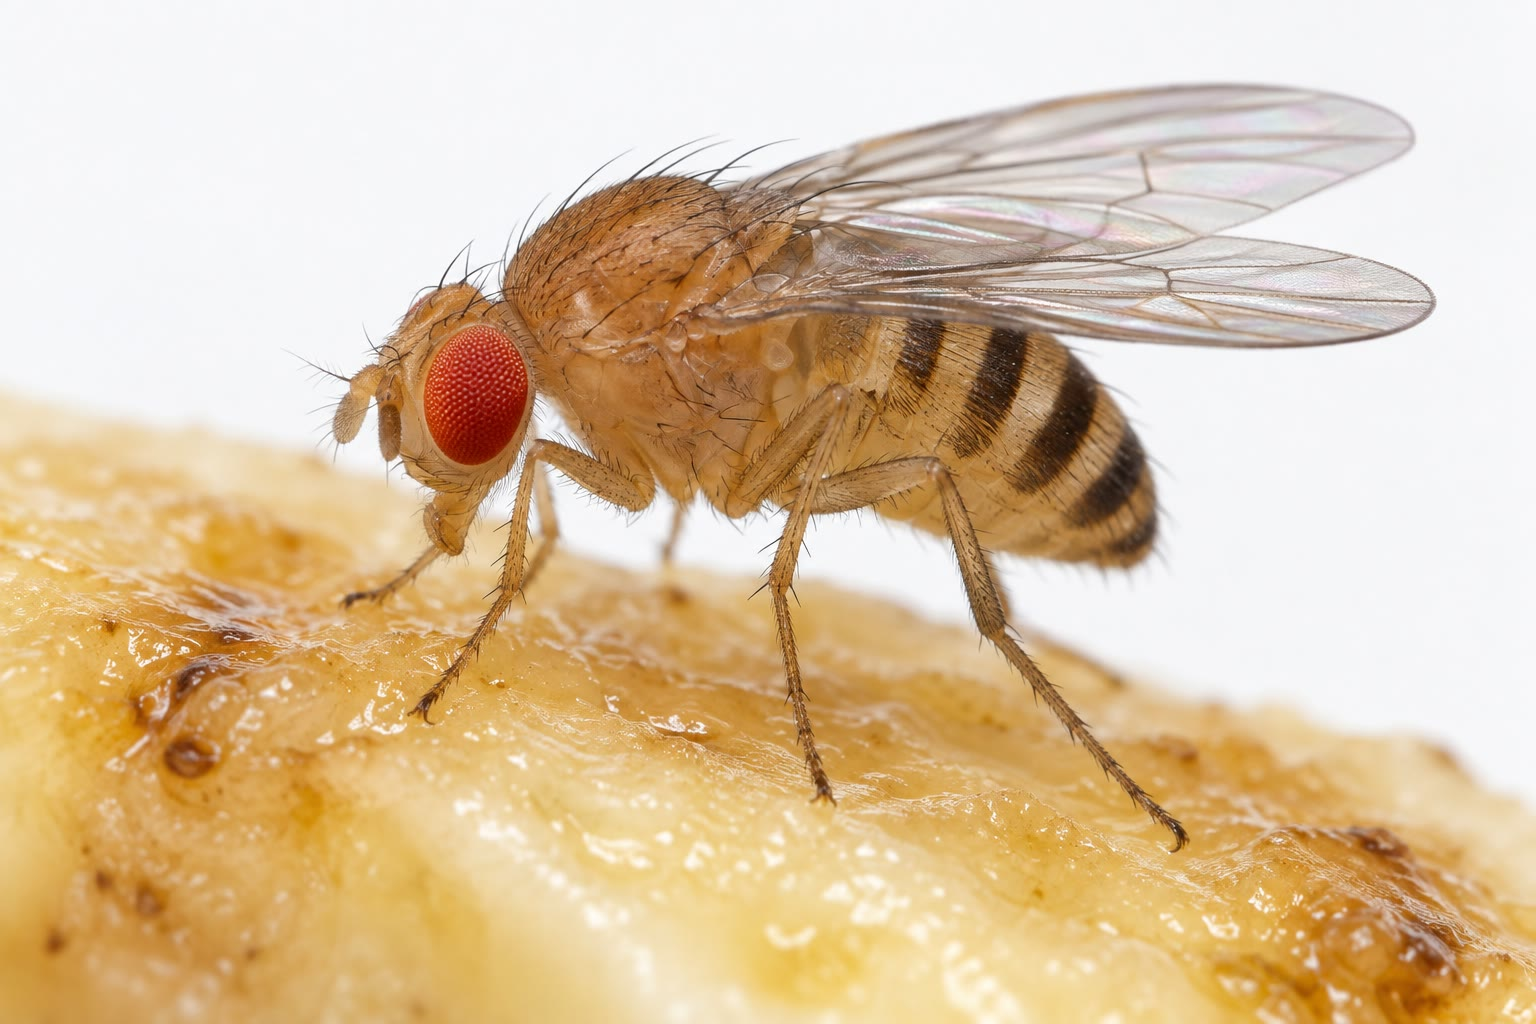
\includegraphics[width=0.5\linewidth]{images/book4/ai/b4-04-drosophila.jpg}

{\small \emph{Drosophila melanogaster}: dua pekan tiap generasi,
ratusan keturunan, empat pasang kromosom, dan seabad mutan --- organisme
yang di atasnya \omterm{def:b2:meiosis-heredity:linkage}{pautan}, peta, dan pewarisan terpaut kelamin
dipecahkan.}
\end{omfigure}

\section{Kromosom kelamin dan organel}

\begin{proposition}[Pewarisan terpaut kelamin]\label{prop:b2:meiosis-heredity:sexlinked}
\index{pewarisan terpaut X}\index{kromosom kelamin}
Pada mamalia dan lalat, betinanya $XX$ dan jantannya $XY$: $Y$-nya
mengusung sedikit gen, sehingga seekor jantan memiliki satu salinan
tiap gen terpaut $X$ (ia \emph{hemizigot}) dan menampakkan \omterm{def:b2:meiosis-heredity:vocabulary}{alel} apa pun
yang diusungnya, \omterm{def:b2:meiosis-heredity:vocabulary}{dominan} maupun \omterm{def:b2:meiosis-heredity:vocabulary}{resesif}. Akibatnya: persilangan timbal
baliknya berbeda (betina bermata putih $\times$ jantan bermata merah
memberi anak jantan bermata putih dan anak betina bermata merah;
persilangan sebaliknya memberi semuanya merah); sebuah ciri \omterm{def:b2:meiosis-heredity:vocabulary}{resesif}
terpaut $X$ (buta warna merah--hijau, hemofilia, distrofi otot
Duchenne) kebanyakan muncul pada jantan, diturunkan induk betina
pembawa yang tidak terkena, dan tidak pernah diturunkan dari ayah
kepada anak jantan (seorang anak jantan memperoleh $Y$ ayahnya);
seorang ayah menurunkan $X$-nya kepada semua anak betinanya. Burung,
kupu-kupu, dan sebagian reptil membalik susunannya (betina $ZW$,
jantan $ZZ$); banyak reptil membiarkan suhu yang memutuskan; dan pada
mamalia satu $X$ tiap sel betinanya dibungkam secara acak pada awal
perkembangannya, sehingga betina \omterm{def:b2:meiosis-heredity:vocabulary}{heterozigot} menjadi sebuah mosaik
(kucing belang tiga).
\end{proposition}
\begin{proof}[Bukti eksperimental]
Morgan (1910) mendapati satu jantan bermata putih di antara ribuan
lalat bermata merah. Disilangkan kepada betina merah, seluruh
keturunannya merah; tetapi pada generasi berikutnya mata putihnya
muncul kembali hanya pada jantan, separuhnya. Menyilangkan jantan putih
kepada anak-anak betinanya yang merah memberi mata putih pada kedua
kelaminnya. Polanya persis seperti yang diharapkan kalau gennya duduk
pada kromosom X, yang diusung betina dua kali dan jantan sekali ---
gen pertama yang ditempatkan pada sebuah kromosom.
\end{proof}

\begin{omfigure}
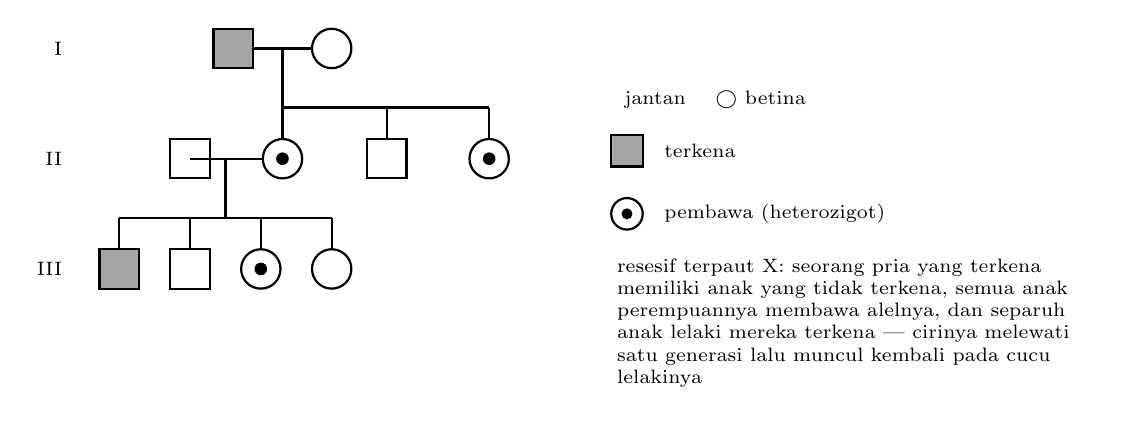
\begin{tikzpicture}[every node/.style={font=\scriptsize}]
  % pedigree: X-linked recessive
  \draw[thick, fill=gray!70] (0,0) rectangle (0.5,0.5); % affected grandfather
  \draw[thick] (1.5,0.25) circle (0.25);
  \draw[thick] (0.5,0.25) -- (1.25,0.25);
  \draw[thick] (0.875,0.25) -- (0.875,-0.5);
  \draw[thick] (0.875,-0.5) -- (3.5,-0.5);
  % children of generation I
  \draw[thick] (0.875,-0.5) -- (0.875,-0.9); \draw[thick, fill=white] (0.875,-1.15) circle (0.25); \fill (0.875,-1.15) circle (0.08);
  \draw[thick] (2.2,-0.5) -- (2.2,-0.9); \draw[thick] (1.95,-1.4) rectangle (2.45,-0.9);
  \draw[thick] (3.5,-0.5) -- (3.5,-0.9); \draw[thick, fill=white] (3.5,-1.15) circle (0.25); \fill (3.5,-1.15) circle (0.08);
  % carrier daughter marries
  \draw[thick] (-0.3,-1.15) -- (0.625,-1.15); \draw[thick] (-0.55,-1.4) rectangle (-0.05,-0.9);
  \draw[thick] (0.15,-1.15) -- (0.15,-1.9); \draw[thick] (-1.2,-1.9) -- (1.5,-1.9);
  \draw[thick] (-1.2,-1.9) -- (-1.2,-2.3); \draw[thick, fill=gray!70] (-1.45,-2.8) rectangle (-0.95,-2.3);
  \draw[thick] (-0.3,-1.9) -- (-0.3,-2.3); \draw[thick] (-0.55,-2.8) rectangle (-0.05,-2.3);
  \draw[thick] (0.6,-1.9) -- (0.6,-2.3); \draw[thick, fill=white] (0.6,-2.55) circle (0.25); \fill (0.6,-2.55) circle (0.08);
  \draw[thick] (1.5,-1.9) -- (1.5,-2.3); \draw[thick, fill=white] (1.5,-2.55) circle (0.25);
  \node[anchor=east] at (-1.8,0.25) {I};
  \node[anchor=east] at (-1.8,-1.15) {II};
  \node[anchor=east] at (-1.8,-2.55) {III};
  % legend
  \node[anchor=west, align=left] at (5,-0.4) {$\square$ jantan \quad $\bigcirc$ betina};
  \draw[thick, fill=gray!70] (5.05,-1.25) rectangle (5.45,-0.85); \node[anchor=west] at (5.6,-1.05) {terkena};
  \draw[thick] (5.25,-1.85) circle (0.2); \fill (5.25,-1.85) circle (0.07); \node[anchor=west] at (5.6,-1.85) {pembawa (heterozigot)};
  \node[anchor=north west, align=left, text width=6.2cm] at (5,-2.3) {resesif terpaut X: seorang pria yang terkena memiliki anak yang tidak terkena, semua anak perempuannya membawa alelnya, dan separuh anak lelaki mereka terkena --- cirinya melewati satu generasi lalu muncul kembali pada cucu lelakinya};
\end{tikzpicture}

{\small Sebuah silsilah ciri \omterm{def:b2:meiosis-heredity:vocabulary}{resesif} terpaut X seperti
hemofilia: tanpa penurunan dari ayah kepada anak lelaki, dengan anak
perempuan pembawa, dan cucu lelaki yang terkena.}
\end{omfigure}

\begin{method}[Membaca sebuah silsilah]\label{met:b2:meiosis-heredity:pedigree}
\index{silsilah}
\begin{enumerate}
  \item Dua orang tua yang tidak terkena dengan seorang anak yang
        terkena: cirinya \omterm{def:b2:meiosis-heredity:vocabulary}{resesif} (kedua tetuanya \omterm{def:b2:meiosis-heredity:vocabulary}{heterozigot}).
  \item Seorang anak yang terkena selalu memiliki tetua yang terkena,
        dan cirinya muncul pada tiap generasi: \omterm{def:b2:meiosis-heredity:vocabulary}{dominan}.
  \item Individu yang terkena kebanyakan lelaki, diturunkan lewat ibu
        yang tidak terkena, tidak pernah dari ayah kepada anak
        lelakinya: \omterm{def:b2:meiosis-heredity:vocabulary}{resesif} terpaut X.
  \item Seorang ayah yang terkena memiliki semua anak perempuan yang
        terkena dan tidak ada anak lelaki yang terkena: \omterm{def:b2:meiosis-heredity:vocabulary}{dominan}
        terpaut X.
  \item Diturunkan oleh ibu kepada semua anaknya, tidak pernah oleh
        ayah: mitokondria.
  \item Lalu hitunglah peluangnya dari \omterm{def:b2:meiosis-heredity:vocabulary}{genotipe} yang tersirat:
        pasangan pembawa $\times$ normal memiliki peluang $\tfrac14$
        memperoleh anak lelaki yang terkena pada tiap kelahiran
        ($\tfrac12$ lelaki $\times$ $\tfrac12$ menerima \omterm{def:b2:meiosis-heredity:vocabulary}{alelnya}).
\end{enumerate}
\end{method}

\begin{definition}[Pewarisan di luar inti]\label{def:b2:meiosis-heredity:extranuclear}
\index{pewarisan maternal}\index{pewarisan mitokondria}
Mitokondria dan kloroplas mengusung genomnya sendiri yang kecil, dalam
banyak salinan tiap organel dan banyak organel tiap sel, dan hampir
seluruhnya datang dari sel telurnya: spermanya menyumbang sebuah
nukleus dan sedikit saja selebihnya. Maka gennya \emph{diwarisi secara
maternal}, tanpa nisbah pemilahan: seorang ibu menurunkan cirinya
kepada semua anaknya, seorang ayah kepada tak seorang pun. Penyakit
mitokondria manusia (cacat rantai respirasi yang mengenai otot dan
saraf) mengikuti pola ini, demikian pula belang-belang sebagian
tumbuhan, tempat sebuah sel induk yang memuat kloroplas normal sekaligus
mutan memilahnya secara acak ke dalam sel anaknya, sehingga
menghasilkan juring hijau, putih, dan campuran. Karena tidak pernah
berekombinasi, urutan mitokondria menjejaki garis keturunan ibu mundur
sepanjang waktu --- alat \cref{ch:b2:phylogenetic-trees}.
\end{definition}

\begin{proposition}[Analisis tetrad]\label{prop:b2:meiosis-heredity:tetrads}
\index{analisis tetrad}\index{tetrad terurut}
Pada sebagian fungi (\emph{Neurospora}, \emph{Sordaria}) keempat hasil
satu \omterm{def:b2:meiosis-heredity:meiosis}{meiosis} tinggal bersama di dalam sebuah kantung, yaitu
\emph{askus}, dan dalam urutan tertentu: sebuah mitosis akhir memberi
delapan spora yang urutannya merekam kedua pembelahannya. Bagi sebuah
\omterm{def:b2:meiosis-heredity:vocabulary}{heterozigot} $A/a$, sebuah askus berpola
$4 : 4$ (\emph{pemilahan pembelahan pertama}) tidak mengalami \omterm{prop:b2:meiosis-heredity:stages}{pindah
silang} antara gennya dan sentromernya --- \omterm{def:b2:meiosis-heredity:vocabulary}{alelnya} berpisah pada anafase
I; sebuah pola $2 : 2 : 2 : 2$ atau $2 : 4 : 2$ (\emph{pemilahan
pembelahan kedua}) mengalami satu \omterm{prop:b2:meiosis-heredity:stages}{pindah silang}, sehingga \omterm{def:b2:meiosis-heredity:vocabulary}{alelnya} baru
berpisah pada anafase II. Jarak dari gennya ke sentromernya adalah
separuh persentase askus pembelahan keduanya, karena sebuah \omterm{prop:b2:meiosis-heredity:stages}{pindah
silang} hanya merekombinasikan dua dari empat kromatidnya. Tetrad juga
menunjukkan secara langsung bahwa rekombinasinya timbal balik: tiap
kromatid rekombinan memiliki pasangan pelengkapnya di dalam askus yang
sama.
\end{proposition}

\begin{omfigure}
\begin{tikzpicture}[every node/.style={font=\scriptsize}]
  \foreach \dx/\pat/\lab in {0/{omDef,omDef,omDef,omDef,omThm,omThm,omThm,omThm}/{$4:4$, tanpa pindah\\silang: pemilahan\\belahan pertama}, 4.5/{omDef,omDef,omThm,omThm,omDef,omDef,omThm,omThm}/{$2:2:2:2$, pindah silang antara\\gen dan sentromernya}, 9/{omDef,omDef,omThm,omThm,omThm,omThm,omDef,omDef}/{$2:4:2$, pindah silang:\\pemilahan belahan kedua}} {
    \begin{scope}[xshift=\dx cm]
      \draw[thick, rounded corners=6pt] (0,0) rectangle (0.8,4.2);
      \foreach \c [count=\i] in \pat { \fill[\c] (0.4,4.2-0.5*\i+0.02) circle (0.2); }
      \node[below, align=center] at (0.4,-0.1) {\lab};
    \end{scope}
  }
  \node[anchor=west, align=left, text width=2.6cm] at (12.4,3.2) {askus terurut \emph{Sordaria}; spora biru dan merah mengusung kedua alelnya};
\end{tikzpicture}

{\small \omterm{prop:b2:meiosis-heredity:tetrads}{Tetrad terurut}. Tanpa \omterm{prop:b2:meiosis-heredity:stages}{pindah silang} antara gennya dan
sentromernya, \omterm{def:b2:meiosis-heredity:vocabulary}{alelnya} berpisah pada pembelahan pertama dan kedelapan
sporanya terbaca $4 : 4$; dengan satu \omterm{prop:b2:meiosis-heredity:stages}{pindah silang}, mereka berpisah
pada pembelahan kedua dan askusnya terbaca $2 : 2 : 2 : 2$ atau
$2 : 4 : 2$.}
\end{omfigure}

\section{Latihan}

\begin{exercise}[$\star$]\label{exo:b2:meiosis-heredity:1}
Sebutkan empat perbedaan antara mitosis dan \omterm{def:b2:meiosis-heredity:meiosis}{meiosis} (cacah
pembelahannya, pemasangannya, hasilnya, keserupaan genetik hasilnya).
\end{exercise}

\begin{exercise}[$\star$]\label{exo:b2:meiosis-heredity:2}
Berapa banyak gamet yang berbeda kromosomnya yang dapat dibuat
seseorang lewat \omterm{thm:b2:meiosis-heredity:mixing}{pemilahan bebas} semata? Seekor lalat buah ($n = 4$)? Sebatang kacang ercis ($n =
7$)?
\end{exercise}

\begin{exercise}[$\star$]\label{exo:b2:meiosis-heredity:3}
Pada kacang ercis, tinggi ($T$) \omterm{def:b2:meiosis-heredity:vocabulary}{dominan} terhadap kerdil. Berikan nisbah
\omterm{def:b2:meiosis-heredity:vocabulary}{fenotipe} dan \omterm{def:b2:meiosis-heredity:vocabulary}{genotipe} $Tt \times Tt$ dan $Tt \times tt$. Bagaimana Anda
mengetahui apakah sebatang tumbuhan yang tinggi itu $TT$ atau $Tt$?
\end{exercise}

\begin{exercise}[$\star$]\label{exo:b2:meiosis-heredity:4}
Definisikan \omterm{def:b2:meiosis-heredity:linkage}{pautan}, \omterm{def:b2:meiosis-heredity:linkage}{frekuensi rekombinasi}, dan \omterm{def:b2:meiosis-heredity:linkage}{sentimorgan}. Mengapa dua
gen pada kromosom yang sama tetap dapat memilah seolah-olah keduanya
saling bebas?
\end{exercise}

\begin{exercise}[$\star\star$]\label{exo:b2:meiosis-heredity:5}
\omterm{thm:b2:meiosis-heredity:mendel}{Persilangan dihibrid} Mendel memberi $315$ bulat kuning, $108$ bulat
hijau, $101$ berkerut kuning, $32$ berkerut hijau. Ujilah hipotesis $9 : 3 : 3 :
1$ dengan $\chi^2$ (3 derajat kebebasan, nilai kritis $7.81$).
\end{exercise}

\begin{exercise}[$\star\star$]\label{exo:b2:meiosis-heredity:6}
Sebuah dihibrid $AB/ab$ yang disilangujikan memberi $412$ $AB$, $388$
$ab$, $103$ $Ab$, $97$ $aB$. Apakah gennya terpaut? Hitunglah \omterm{def:b2:meiosis-heredity:linkage}{frekuensi
rekombinasi} dan jarak petanya; apa yang akan diberikan dihibrid $Ab/aB$?
\end{exercise}

\begin{exercise}[$\star\star$]\label{exo:b2:meiosis-heredity:7}
Dengan memakai fungsi Haldane, ubahlah $r = 0.20$ dan $r = 0.45$
menjadi jarak peta, serta \qty{30}{cM} dan \qty{100}{cM} menjadi fraksi
rekombinasi. Ulaslah konversi mana yang berarti dalam praktiknya.
\end{exercise}

\begin{exercise}[$\star\star$]\label{exo:b2:meiosis-heredity:8}
Pada \emph{Drosophila}, mata putih ($w$) bersifat \omterm{def:b2:meiosis-heredity:vocabulary}{resesif} terpaut X.
Berikan keturunannya, menurut kelamin dan \omterm{def:b2:meiosis-heredity:vocabulary}{fenotipe}, dari (a) betina
putih $\times$ jantan merah, (b) betina merah \omterm{def:b2:meiosis-heredity:vocabulary}{heterozigot} $\times$
jantan putih, (c) persilangan anak betina (a) dengan saudara jantannya.
\end{exercise}

\begin{exercise}[$\star\star$]\label{exo:b2:meiosis-heredity:9}
Dua galur murni kacang manis berbunga putih, ketika disilangkan,
memberi keturunan semuanya ungu, yang kalau diserbuki sendiri memberi
$9$ ungu : $7$ putih. Jelaskan dengan dua gen, berikan \omterm{def:b2:meiosis-heredity:vocabulary}{genotipe} kedua
galur tetuanya, lalu ramalkan hasil penyilangujian hibrid ungunya.
\end{exercise}

\begin{exercise}[$\star\star\star$]\label{exo:b2:meiosis-heredity:10}
Sebuah persilangan uji tiga titik memberi: $+++$ 480, $abc$ 470, $+bc$
11, $a++$ 9, $++c$ 118, $ab+$ 112, $+b+$ 1, $a+c$ 1 (jumlahnya 1202).
Carilah urutan gennya, kedua jaraknya, koefisien kebetulannya, dan
interferensinya.
\end{exercise}

\begin{exercise}[$\star\star\star$]\label{exo:b2:meiosis-heredity:11}
Pada \emph{Sordaria}, persilangan galur berspora hitam dengan galur
berspora cokelat muda memberi $700$ askus berpola $4 : 4$ dan $300$
askus berpola $2 : 2 : 2 : 2$ atau $2 : 4 : 2$. Hitunglah jarak dari
gen warna sporanya ke sentromernya, lalu jelaskan mengapa faktor
setengahnya dibutuhkan. Gambarkanlah kromatid satu \omterm{def:b2:meiosis-heredity:meiosis}{meiosis} yang
memberi $2 : 4 : 2$.
\end{exercise}

\begin{exercise}[$\star\star\star$]\label{exo:b2:meiosis-heredity:12}
Kakek dari pihak ibu seorang perempuan menderita hemofilia; tak seorang
pun lagi di dalam keluarganya yang terkena. Berapa peluang bahwa ia
seorang pembawa? Mengingat ia telah memiliki dua anak lelaki yang
sehat, berapa peluangnya sekarang? Tunjukkan penalarannya.
\end{exercise}

\section{Soal: Persilangan di Ruang Lalat}

\begin{problem}[{Soal akhir pekan --- persilangan \emph{Drosophila}
dianalisis dari nisbah monohibrid sampai peta tiga titik, dan sebuah
silsilah manusia dihitung, berakhir pada peta tiga gen terpaut X dan
interferensinya}]
\label{pb:b2:meiosis-heredity:1}
Sayap vestigial ($vg$) dan tubuh eboni ($e$) bersifat \omterm{def:b2:meiosis-heredity:vocabulary}{resesif} dan
terletak pada autosom yang berbeda; tubuh hitam ($b$) dan $vg$ bersifat
\omterm{def:b2:meiosis-heredity:vocabulary}{resesif} dan keduanya terletak pada kromosom 2; tubuh kuning ($y$), mata
putih ($w$), dan sayap mungil ($m$) bersifat \omterm{def:b2:meiosis-heredity:vocabulary}{resesif} dan terpaut X.
Nilai kritis $\chi^2$ pada \qty{5}{\%}: $3.84$ (1 d.b.), $7.81$ (3 d.b.).

\medskip
\noindent\textbf{Bagian I --- Dua gen autosom.}
Seekor lalat vestigial murni disilangkan kepada seekor lalat eboni
murni; $F_1$-nya seluruhnya tipe liar; $1600$ lalat $F_2$ dinilai:
$892$ liar, $309$ vestigial, $296$ eboni, $103$ vestigial eboni.
\begin{enumerate}
  \item Berikan \omterm{def:b2:meiosis-heredity:vocabulary}{genotipe} tetuanya, \omterm{def:b2:meiosis-heredity:vocabulary}{genotipe} $F_1$-nya, dan gamet
        $F_1$-nya.
  \item Hitunglah cacah harapannya di bawah \omterm{thm:b2:meiosis-heredity:mixing}{pemilahan bebas}.
  \item Hitunglah $\chi^2$ lalu simpulkan.
  \item Berapa bagian lalat $F_2$ bertipe liar yang \omterm{def:b2:meiosis-heredity:vocabulary}{homozigot} pada
        kedua lokusnya?
  \item $F_1$-nya disilangujikan kepada seekor lalat vestigial eboni:
        ramalkan keempat golongannya dan proporsinya.
  \item Lalat eboni yang dipelihara pada \qty{29}{\celsius} lebih pucat
        daripada pada \qty{18}{\celsius}. Apa yang dikatakannya tentang
        hubungan \omterm{def:b2:meiosis-heredity:vocabulary}{genotipe} dengan \omterm{def:b2:meiosis-heredity:vocabulary}{fenotipe}?
\end{enumerate}

\medskip
\noindent\textbf{Bagian II --- Dua gen yang terpaut.}
Seekor lalat hitam murni disilangkan kepada seekor lalat vestigial
murni; betina $F_1$-nya disilangujikan kepada jantan hitam vestigial:
$965$ hitam, $944$ vestigial, $206$ hitam vestigial, $185$ tipe liar.
\begin{enumerate}[resume]
  \item Tuliskanlah \omterm{def:b2:meiosis-heredity:vocabulary}{genotipe} $F_1$-nya, sambil menunjukkan \omterm{def:b2:meiosis-heredity:vocabulary}{alel} mana
        yang berada pada kromosom yang sama.
  \item Kenalilah golongan tetua dan golongan rekombinannya lalu
        jelaskan mengapa tipe liarnya di sini adalah \emph{rekombinan}.
  \item Hitunglah $r$ dan jarak petanya.
  \item Betulkanlah dengan fungsi Haldane.
  \item Persilangan yang sama dengan \emph{jantan} $F_1$ yang
        disilangujikan hanya memberi dua golongan, hitam dan
        vestigial, sama banyak. Apa yang ditunjukkannya tentang \omterm{def:b2:meiosis-heredity:meiosis}{meiosis}
        pada lalat jantan?
  \item Ramalkanlah golongan dan proporsinya kalau betina $F_1$-nya
        berasal dari persilangan hitam vestigial $\times$ liar.
\end{enumerate}

\medskip
\noindent\textbf{Bagian III --- Sebuah silsilah manusia.}
Hemofilia A bersifat \omterm{def:b2:meiosis-heredity:vocabulary}{resesif} terpaut X. Seorang pria dengan hemofilia
memiliki seorang anak perempuan, yang menikah dengan pria yang tidak terkena.
\begin{enumerate}[resume]
  \item Apakah \omterm{def:b2:meiosis-heredity:vocabulary}{genotipe} anak perempuannya, dan mengapa \omterm{def:b2:meiosis-heredity:vocabulary}{genotipe} itu pasti?
  \item Peluang bahwa anak pertamanya adalah anak lelaki yang terkena.
  \item Peluang bahwa seorang anak perempuannya adalah pembawa.
  \item Peluang bahwa, di antara ketiga anaknya, tak seorang pun
        terkena.
  \item Jelaskan mengapa penyakitnya tidak pernah diturunkan dari ayah
        kepada anak lelaki, dan bagaimana seorang perempuan dapat terkena.
  \item Saudara perempuan pria yang terkena itu memiliki dua anak
        lelaki yang sehat; ibu mereka (ibu pria itu) adalah seorang
        pembawa. Hitunglah peluang bahwa saudara perempuannya adalah
        pembawa, sebelum dan sesudah memperhitungkan anak lelakinya.
\end{enumerate}

\medskip
\noindent\textbf{Bagian IV --- Tiga gen terpaut X.}
Seekor betina $y\,w\,m/+\,+\,+$ disilangkan kepada seekor jantan
$y\,w\,m$; $2000$ anak jantannya dinilai: $+++$ 853, $ywm$ 833, $y++$
24, $+wm$ 26, $yw+$ 128, $++m$ 132, $+w+$ 2, $y+m$ 2.
\begin{enumerate}[resume]
  \item Mengapa anak jantannya dapat dinilai langsung, tanpa sebuah
        persilangan uji?
  \item Kenalilah golongan tetua dan golongan \omterm{prop:b2:meiosis-heredity:stages}{pindah silang} gandanya
        lalu simpulkan urutan gennya.
  \item Hitunglah kedua \omterm{def:b2:meiosis-heredity:linkage}{frekuensi rekombinasinya} lalu gambarkan petanya.
  \item Hitunglah harapan cacah \omterm{prop:b2:meiosis-heredity:stages}{pindah silang} gandanya, koefisien
        kebetulannya, dan interferensinya.
  \item Hitunglah \omterm{def:b2:meiosis-heredity:linkage}{frekuensi rekombinasi} antara kedua gen terluarnya
        langsung dari datanya, lalu jelaskan mengapa nilainya lebih
        kecil daripada jumlah kedua jaraknya.
  \item Akan tampak seperti apa anak betina persilangan ini, dan
        mengapa mereka tidak berguna untuk pemetaan?
  \item Nyatakan hasilnya: peta ketiga gennya dan interferensinya.
\end{enumerate}
\end{problem}
